\chapter{Experiments on Double Descent}
\label{experimental_part}

In this chapter, several experiments on generalization of neural networks will be done. The main goal is to demonstrate and explore the double descent risk curve. It shall be discovered, how far the risk curve can be predicted or influenced. The hope is that conclusions regarding the origin of the double descent risk curve can be drawn from the experiments described and conducted in this chapter.\\
What determines the position of the beginning of the second decrease? How can the peak before the second fall of the curve be influenced? Can a point on the curve after the second decrease be found such that the performance is better then after the first decrease of the curve?  It will also be shown that double descent is independent of the minimization algorithm and the data set.

\section{Experimental Setup}

In order to detect or explore double descent, we need a network in which the number of parameters can be increased step by step. A simple method, even if it may not produce the best generalization, would be a network with a hidden layer, i.e. $L = 1$. This hidden layer contains a variable number of neurons $H$. If more parameters are needed, $H$ can be increased. A similar setup was also used in the paper Reconciling modern machine-learning practice and the classical bias–variance trade-off by Mikhail Belkin \cite{belkin}. The neurons in the hidden layer should have connections to all input neurons and all output neurons. The hidden layer is therefore a dens layer. As activation function of the neurons in the hidden layer the  rectified linear activation function or $ReLU$ shall be used. With,
$$
ReLU(x) := \rho(x) = max(0,x)
$$
For almost all experiments, we will use the MNIST dataset, which consists of $60000$ training data and $10000$ Test data \cite{wikipedia_Mnist-Datenbank}. An element from the MNIST set is a greyscale image of a $28 \times 28$ pixel large image, which shows a handwritten number between 0 and 9. The input layer $x$ must therefore have a size of $28 \cdot 28 = 784$. For each pixel one neuron. The training set is normalized before training, so the neurons take a value between $0$ and $1$ as an input depending on the intensity of the represented pixel. The output layer, on the other hand, must have a size of 10 neurons, since we train the model to distinguish between 10 different classes. The activation function for the output layer should be the softmax function $\sigma$, which is given by,
$$
\sigma : \mathbb{R}^{10} \xrightarrow{} [0,1]^{10} \text{ with } \sigma(z)_i = \frac{e^{z_i}}{\sum_{j = 1}^{10}e^{z_j}}.
$$

\begin{figure}
\centering
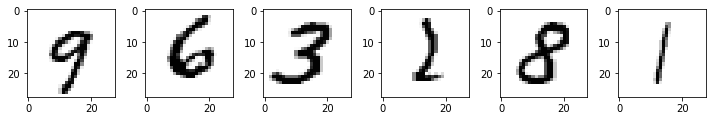
\includegraphics[width= 1\linewidth]{Abschlussarbeit_2021/LaTeX/images/MNIST.png}
\caption{ Six examples of the Trainingset of MNIST}
\end{figure}

The output value of the function is then an array of length 10, where the i-th entry contains the probability for class i. Let $y$ be the output of the output layer so the classification of the input is given by $y_i = \arg\max_{i \in \{1, \cdots,10\}}(y)$. \\
The model $M$ which is used in the following experiments can thus be represented mathematically by,
\begin{equation}
    M(x) = \arg\max(\sigma_0, \cdots \sigma_9) \\
    \text{ with } \sigma_k = [\sum_{i = 1}^H w^{(2)}_{i,k} \cdot \rho(\sum_{j=1}^{784}w^{(1)}_{j,i}\cdot x_j) + b^{(1)}_i] + b^{(2)}_k
    \label{model equation}
\end{equation}

Where $w^{(1)} \in \mathbb{R}^{784 \times H}$ is the weight matrix between the input layer and the hidden layer and $w^{(2)} \in \mathbb{R}^{H \times 10}$ is the weight matrix between the hidden layer and the output layer. The bias vector for the hidden layer is $b^{(1)}$. $b^{(2)}$ is the bias vector from the output layer. All weights in the weight matrices and all biases in the layers should be allowed to change through the optimization process. The number of parameters that can be trained depends only on $H$, because input and output layer always have the same size. The amount of trainable Parameters $P$ is therefore given by,
$$
P(H) = (784+1)\cdot H + (H+1) \cdot 10
$$
As a loss-function, category crossentropy should be used, as it is usual for classification problems. Which is given by,
\begin{equation}
    L(x) =  - \sum_{i = 0}^{9} y_i^* \cdot \log y_i
    \label{scc_eq}
\end{equation}
where $y = [y_0,y_1 \cdots, y_9] = M(x)$ is the output of the model in equation 2.1, whereas $y^* =[y^*_0,y^*_1 \cdots, y^*_9]$ is the target value i.e how the model should react. For example if the label of a point $x$ is $4$, $y^*$ would be $[0,0,0,0,1,0,0,0,0,0]$. \\
To minimize the loss function $L(x)$ stochastic gradient descent (SGD) is used. This is done by updating the weights and biases into the direction of the approximated gradient.
$$
w_{i,j}^{(n+1)} := w_{i,j}^{(n)}  - \eta \frac{\delta L}{\delta w_{i,j}}
$$
%%TODO: OPTIMIZE Formula. 
%%%%%%%%%%%%%%%%%%%%%%%%%%%
%%%%%%%%%%%%%%%%%%%%%%%
%%TODO!!!!!!!!!!!!!!!!!!!!!!

where $w_{i,j}^{(n)}$ is the weight matrix at $i,j$ at iteration $n$. The same rule holds for the biases. $\eta$ is the learning rate or the stepsize. In the following experiments a learning rate $\eta = 0.05$ will be used. By minimizing the loss function the model performs better and better on training data. \\
In the introduction, the question was asked why, despite a loss function that assumes extremely low values in the training data, a network still performs very well. That is why an extremely small training loss is always achieved during training from a certain model size.



\newpage

\section{Experiments}

Before more complex experiments are performed, the existence of the double descent curve described in Beklin's paper should be empirically proven. For this purpose a model $M$ from equation \ref{model equation} is taken. $M$ is thereby supposed to have $1 \leq H \leq 80$ neurons. Thus, a total of 80 training sessions are run. The training and test loss is measured at each iteration of $H$. The training process is stopped when either $200$ epochs have been reached or a test-loss below $0.001$ has been reached. $M$ was trained on a subset of MNIST with $20000$ Samples. It could be argued that stopping earlier for large networks contributes to the second drop of the curve, since this way overfitting is no longer done. However, this is not the case. Stopping at a certain test loss is only done to save time. Figure \ref{fig:epochs_double_descent} shows double descent curves, where independent of the model size always the same number of epochs was run through. This curve looks very similar to the one in Figure \ref{double_descent_vanilla}.

\begin{figure}[!htp]
\centering
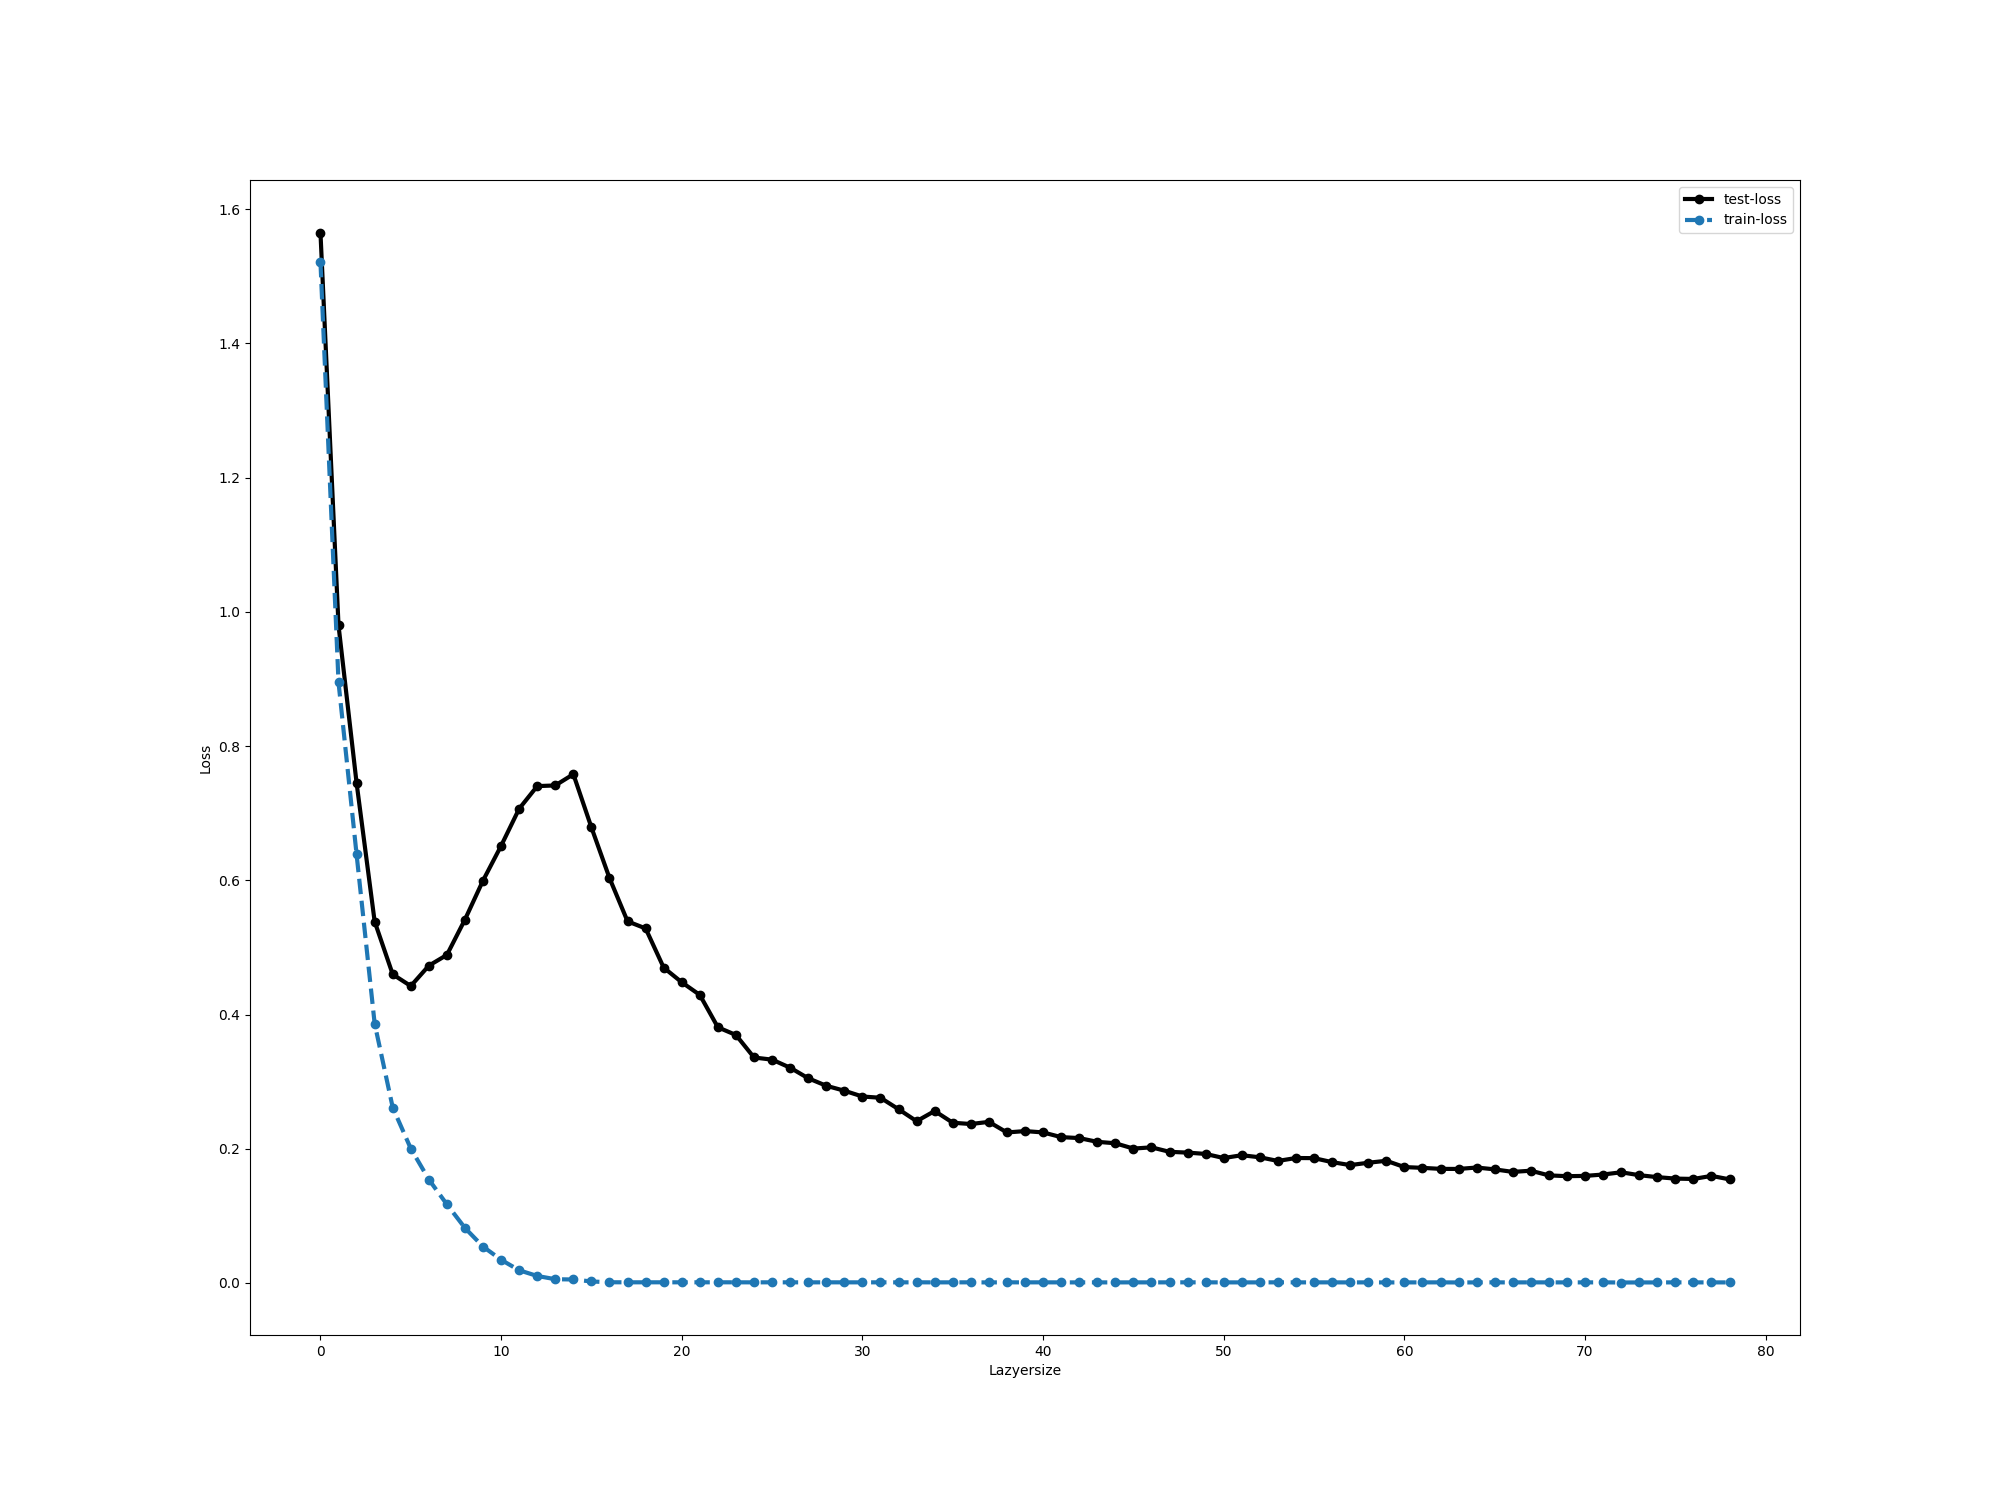
\includegraphics[width= 1\linewidth]{Abschlussarbeit_2021/LaTeX/images/double_sgd.png}
\caption{Train-loss and test-loss averaged over 10 runs}
\label{double_descent_vanilla}
\end{figure}

In Figure \ref{double_descent_vanilla}, two important observations can be made. The first one is that the performance of $M$ is better from a certain number of neurons ($H = 21$) than before the peak. Even if the training was not optimal up to the local maximum, because the model was overfitted with 200 epochs, the generalization is extremely good at $H = 80$. Here a test accuracy of $97\%$ was achieved. 
the second observation that can be made concerns the position of the peak. This can be observed at $H = 16$. The test loss, on the other hand, is zero the first time from $H = 16$. The peak is called \textit{"interpolation threshold"} by Belkin \cite{belkin}. The reason for this is that the data can be interpolated from this point because the model has sufficient capacity. The region to the left of the interpolation threshold is called \textit{"underparameterized regime"} and the region to the right of the interpolation threshold is called \textit{"overparameterized regime"}. overparameterized and underparameterized respectively, because there are more than enough or not enough parameters to learn the training data perfectly.\\
In the further part of the section the effect on the shape of the curve will be tested by changing different attributes. How does the curve behave when changing the sample size? What influence does the number of epochs have? And what happens when the labels are replaced with noise during training?

\subsection{The influence of data quantity}

If the data quantity is reduced or increased, the peak at the interpolation threshold shifts to the left or to the right, respectively. 
This means the model can reach a zero percent test loss faster if the amount of data is smaller. This is a very predictable and logical finding. It is interesting, however, that the statement \textit{"more data is always better"} is not that clear to observe. On the one hand, a model $M_{H=80}$\footnote{Model with $80$ neurons in the hidden layer} trained with 5000 samples and 80 neurons can perform better than a smaller model $M_{H \leq 20}$ with up to 20 neurons trained with 20000 samples.
For large and small $H$, the performance is clearly better when more data was used to train. However, there is a range $(10 \leq H \leq 22)$ where the order of generalization is not entirely clear.\\
This will be discussed in more detail in chapter \ref{train_dd}. For small $H$ with $5 \leq H \leq 10$ and large $23 \leq H $, it is clear that more data improves the generalization. The peaks at the interpolation threshold are somewhat broader for larger data sets.  

\begin{figure}[!htp]
\centering
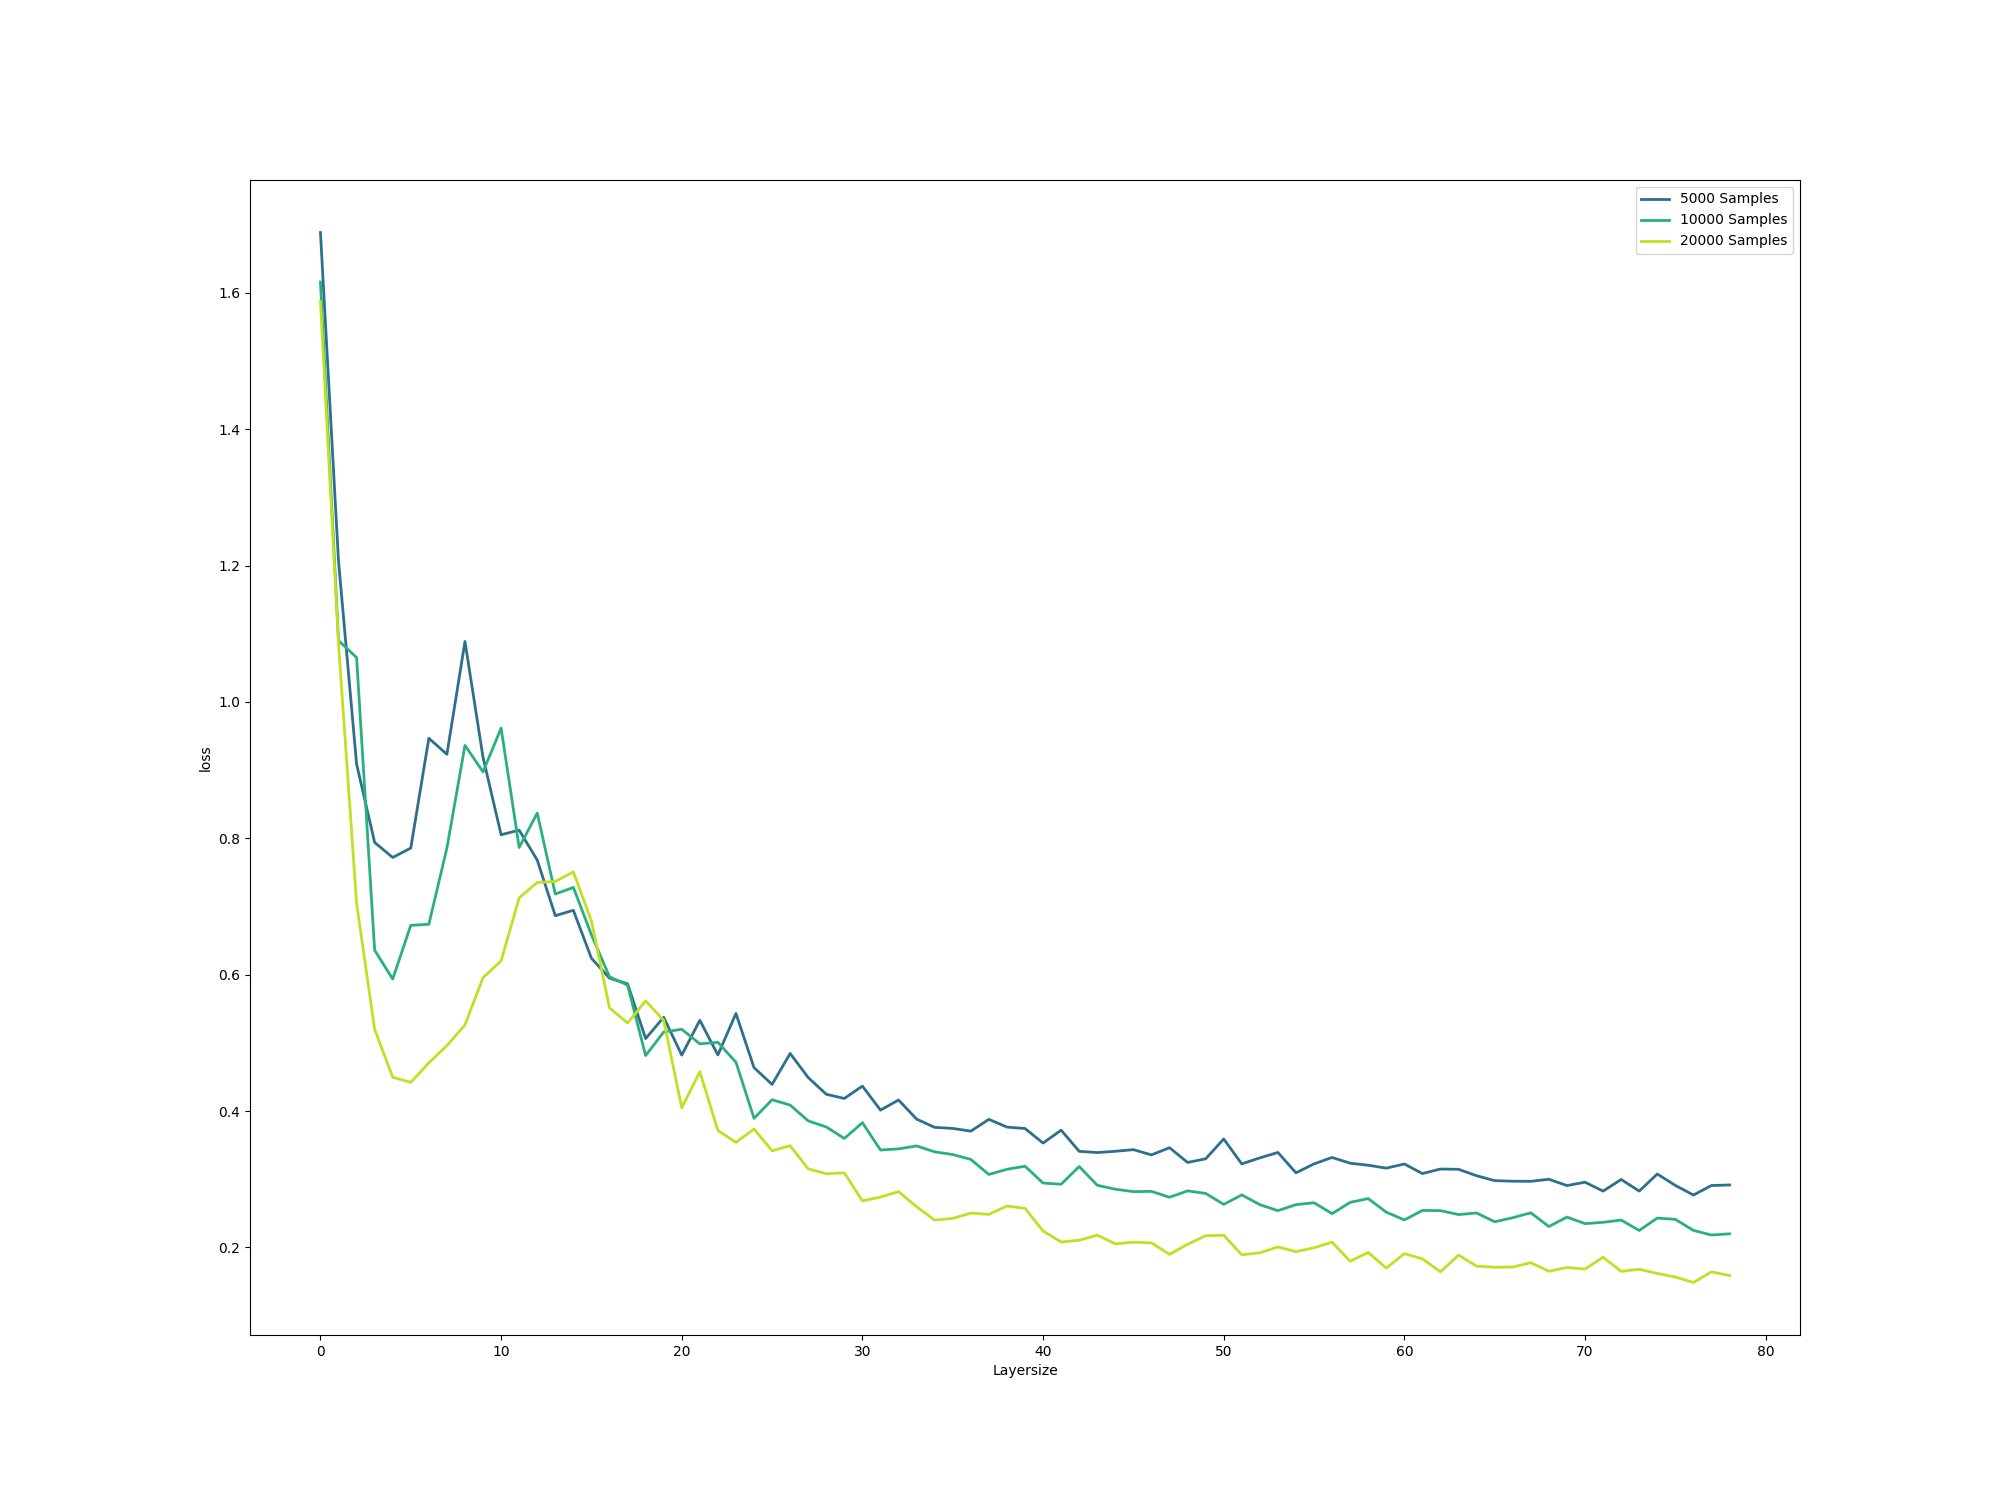
\includegraphics[width= 1\linewidth]{Abschlussarbeit_2021/LaTeX/images/diff_samplesizes.png}
\caption{test-loss averaged over 2 runs. The experiment was performed with 3 different sized subsets of MNIST.}
\label{fig:sample_size_double_descent}
\end{figure}



\subsection{The influence of epochs}


It is known that overfitting can occur when training neural networks by running through too many epochs. The model then can perform worse on unseen data.   



\begin{figure}[!htp]
\centering
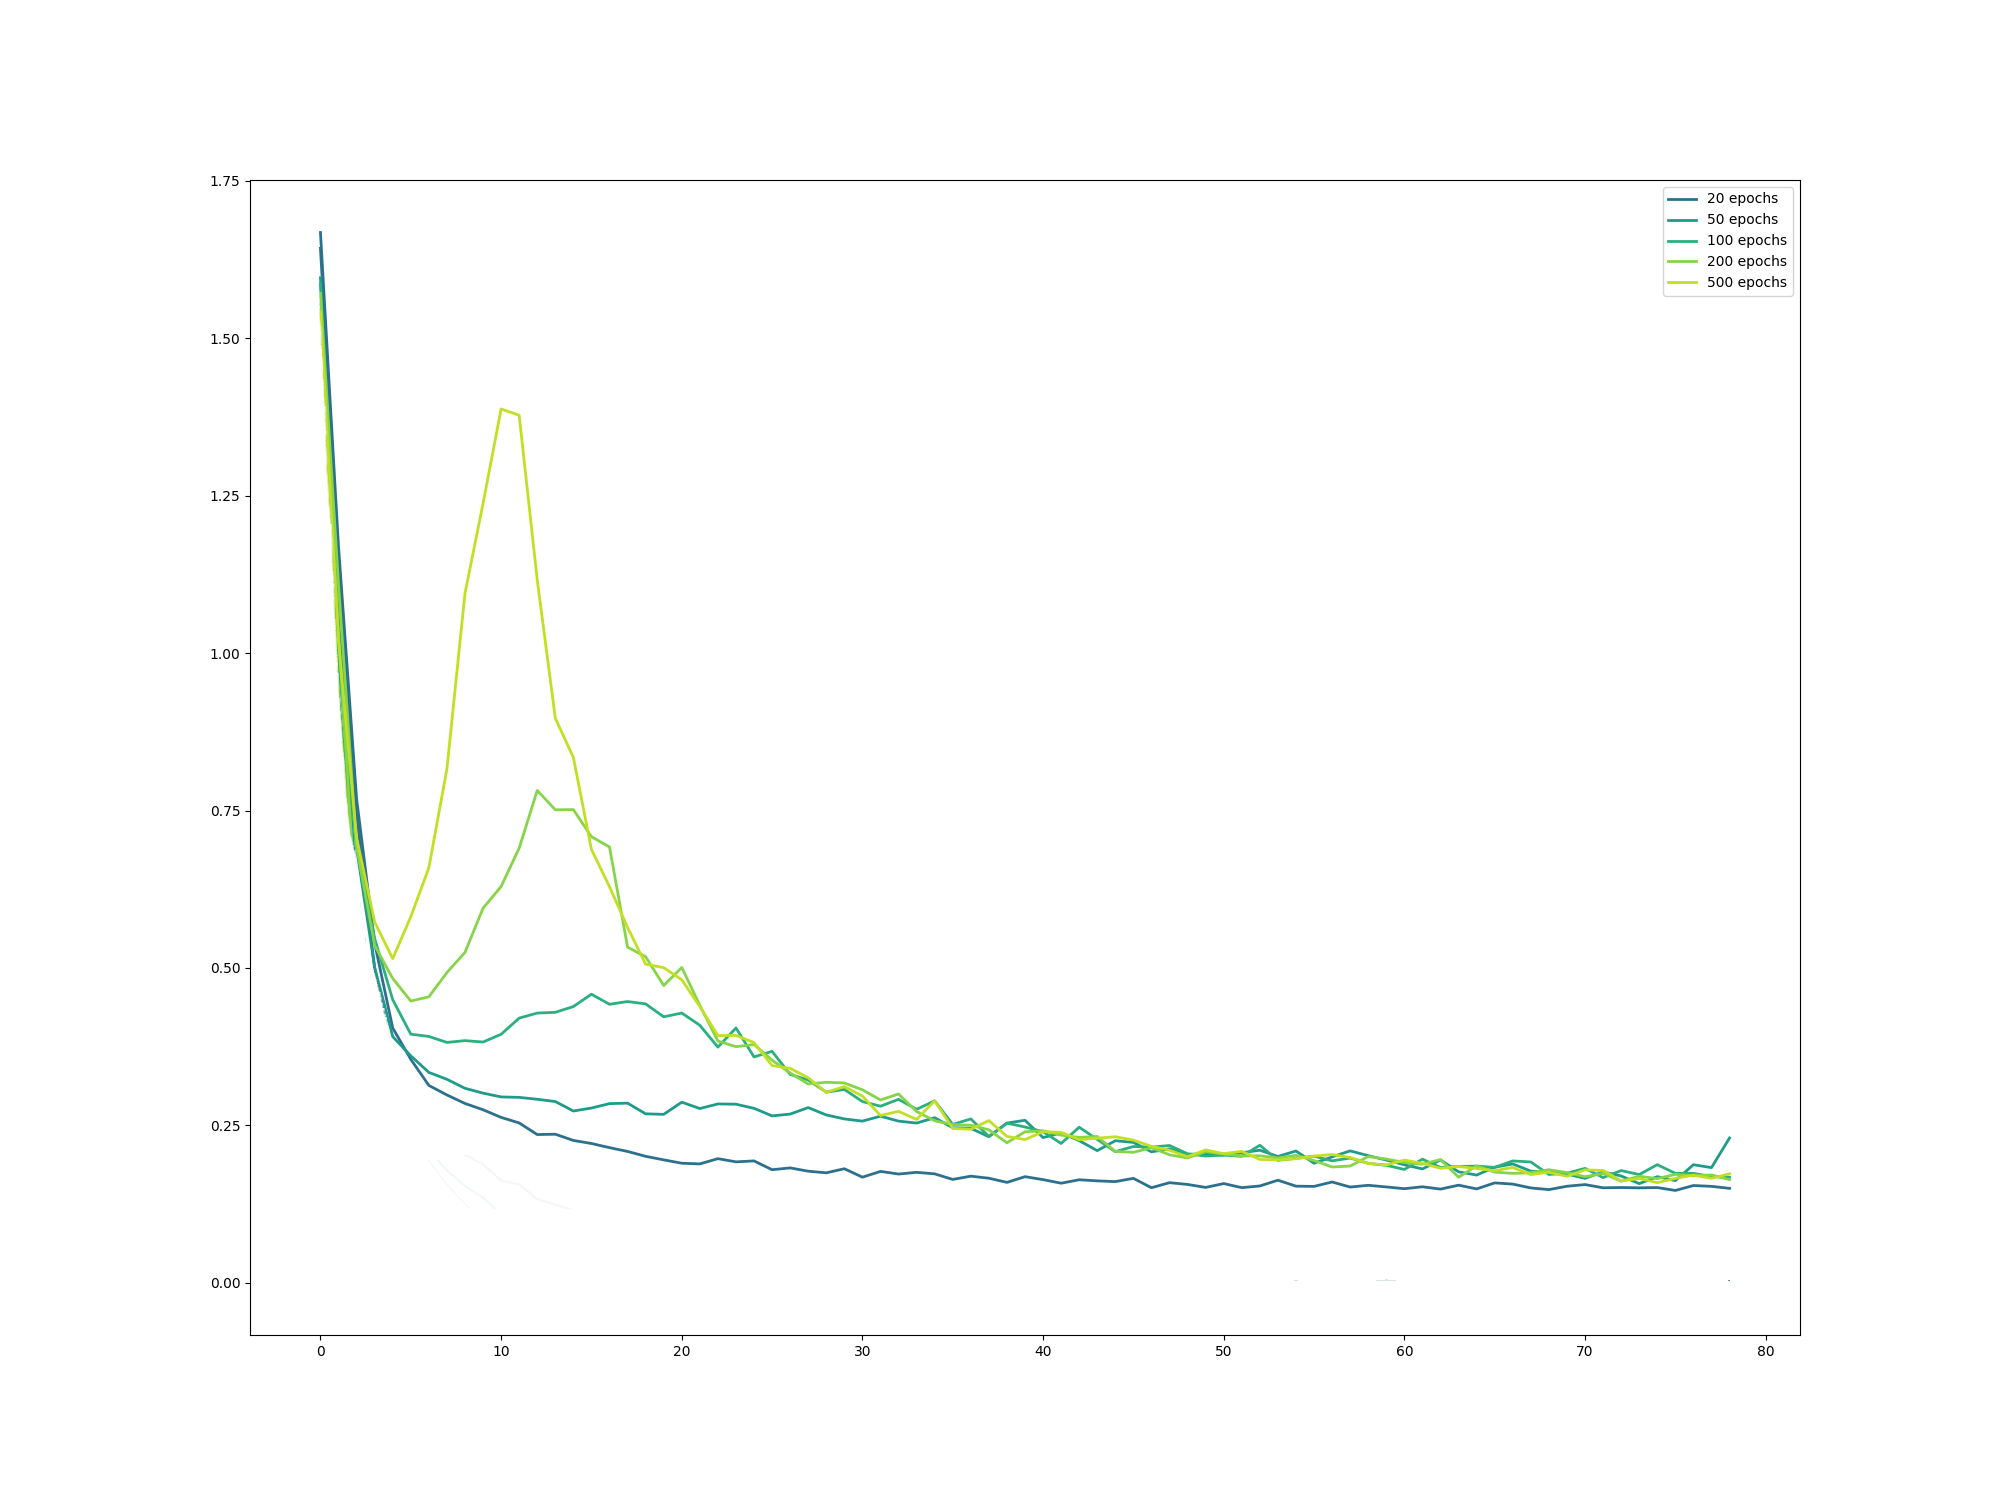
\includegraphics[width= 1\linewidth]{Abschlussarbeit_2021/LaTeX/images/many_epochs.png}
\caption{Test-loss depending on the amount of epochs averaged over 4 runs}
\label{fig:epochs_double_descent}
\end{figure}


Figure \ref{fig:sample_size_double_descent} clearly shows that the number of epochs has a large influence on the peak at the interpolation threshold. The more epochs are passed through, the higher is the peak. 
Double descent can even be completely omitted with the selected architecture if training was carried out with only a few epochs. In addition, the interpolation threshold moves further and further to the left as the number of epochs increases. The perfect interpolation of the data happens already with smaller $H$. This finding is logical, because at certain $H$ after a few epochs no minimum with zero train loss was found, which interpolates the data perfectly. If one would run through more epochs, however, the said minimum can be found.
As mentioned above, the training was not ended prematurely when a certain training loss was reached. The test loss is very similar for all epoch numbers for large $H$. This is also an interesting finding.




\subsection{The influence of noise}

As has already been observed, the train-loss after the interpolation threshold is zero. This means that the data is perfectly memorized. The MNIST data set possesses little noise. Even though some numbers are drawn inaccurately, the label is always appropriate to the image. However, in many more complex applications, there is often a lot of noise in data sets. Labels are sometimes not fitting to the respective data point (label noise). Measured values could also become inaccurate due to different environmental influences. In such cases, is it necessarily wanted that the model learns all its training data perfectly by memory? As will be shown later, noise causes a high variance in the set of possible learned function. This means that if the network is trained more often, the resulting learned functions will be more different from each other. To memorize this noise, the model also needs significantly more capacity. In the case of MNIST, the model could remember that at label $7$ the pixel $(x,y)$ is active. Due to label noise, it can happen that an actual image of a $6$ is labeled as $7$. So the simple constrain $7 \	\Longrightarrow (x,y) > 0.8$ is not sufficient, and the model must find more complex structures to get the label noise under control.\\
The effect can be observed in Figure \ref{fig:Label_noise_on_double_descent}. With increased label noise, the peak at the interpolation threshold is seen much later. In addition, the test loss value is also significantly higher there. However, it can also be assumed that for large $H$ and with not too high label noise, the model performs better in the overparameterized region than in the underparameterized region, since the curves are still decreasing after $H = 80$. For certain $H$ it can even be seen that paradoxically more noise leads to better generalization. This point will be taken up again in \ref{less_noise_can_hurt}. 


\begin{figure}[!htp]
\centering
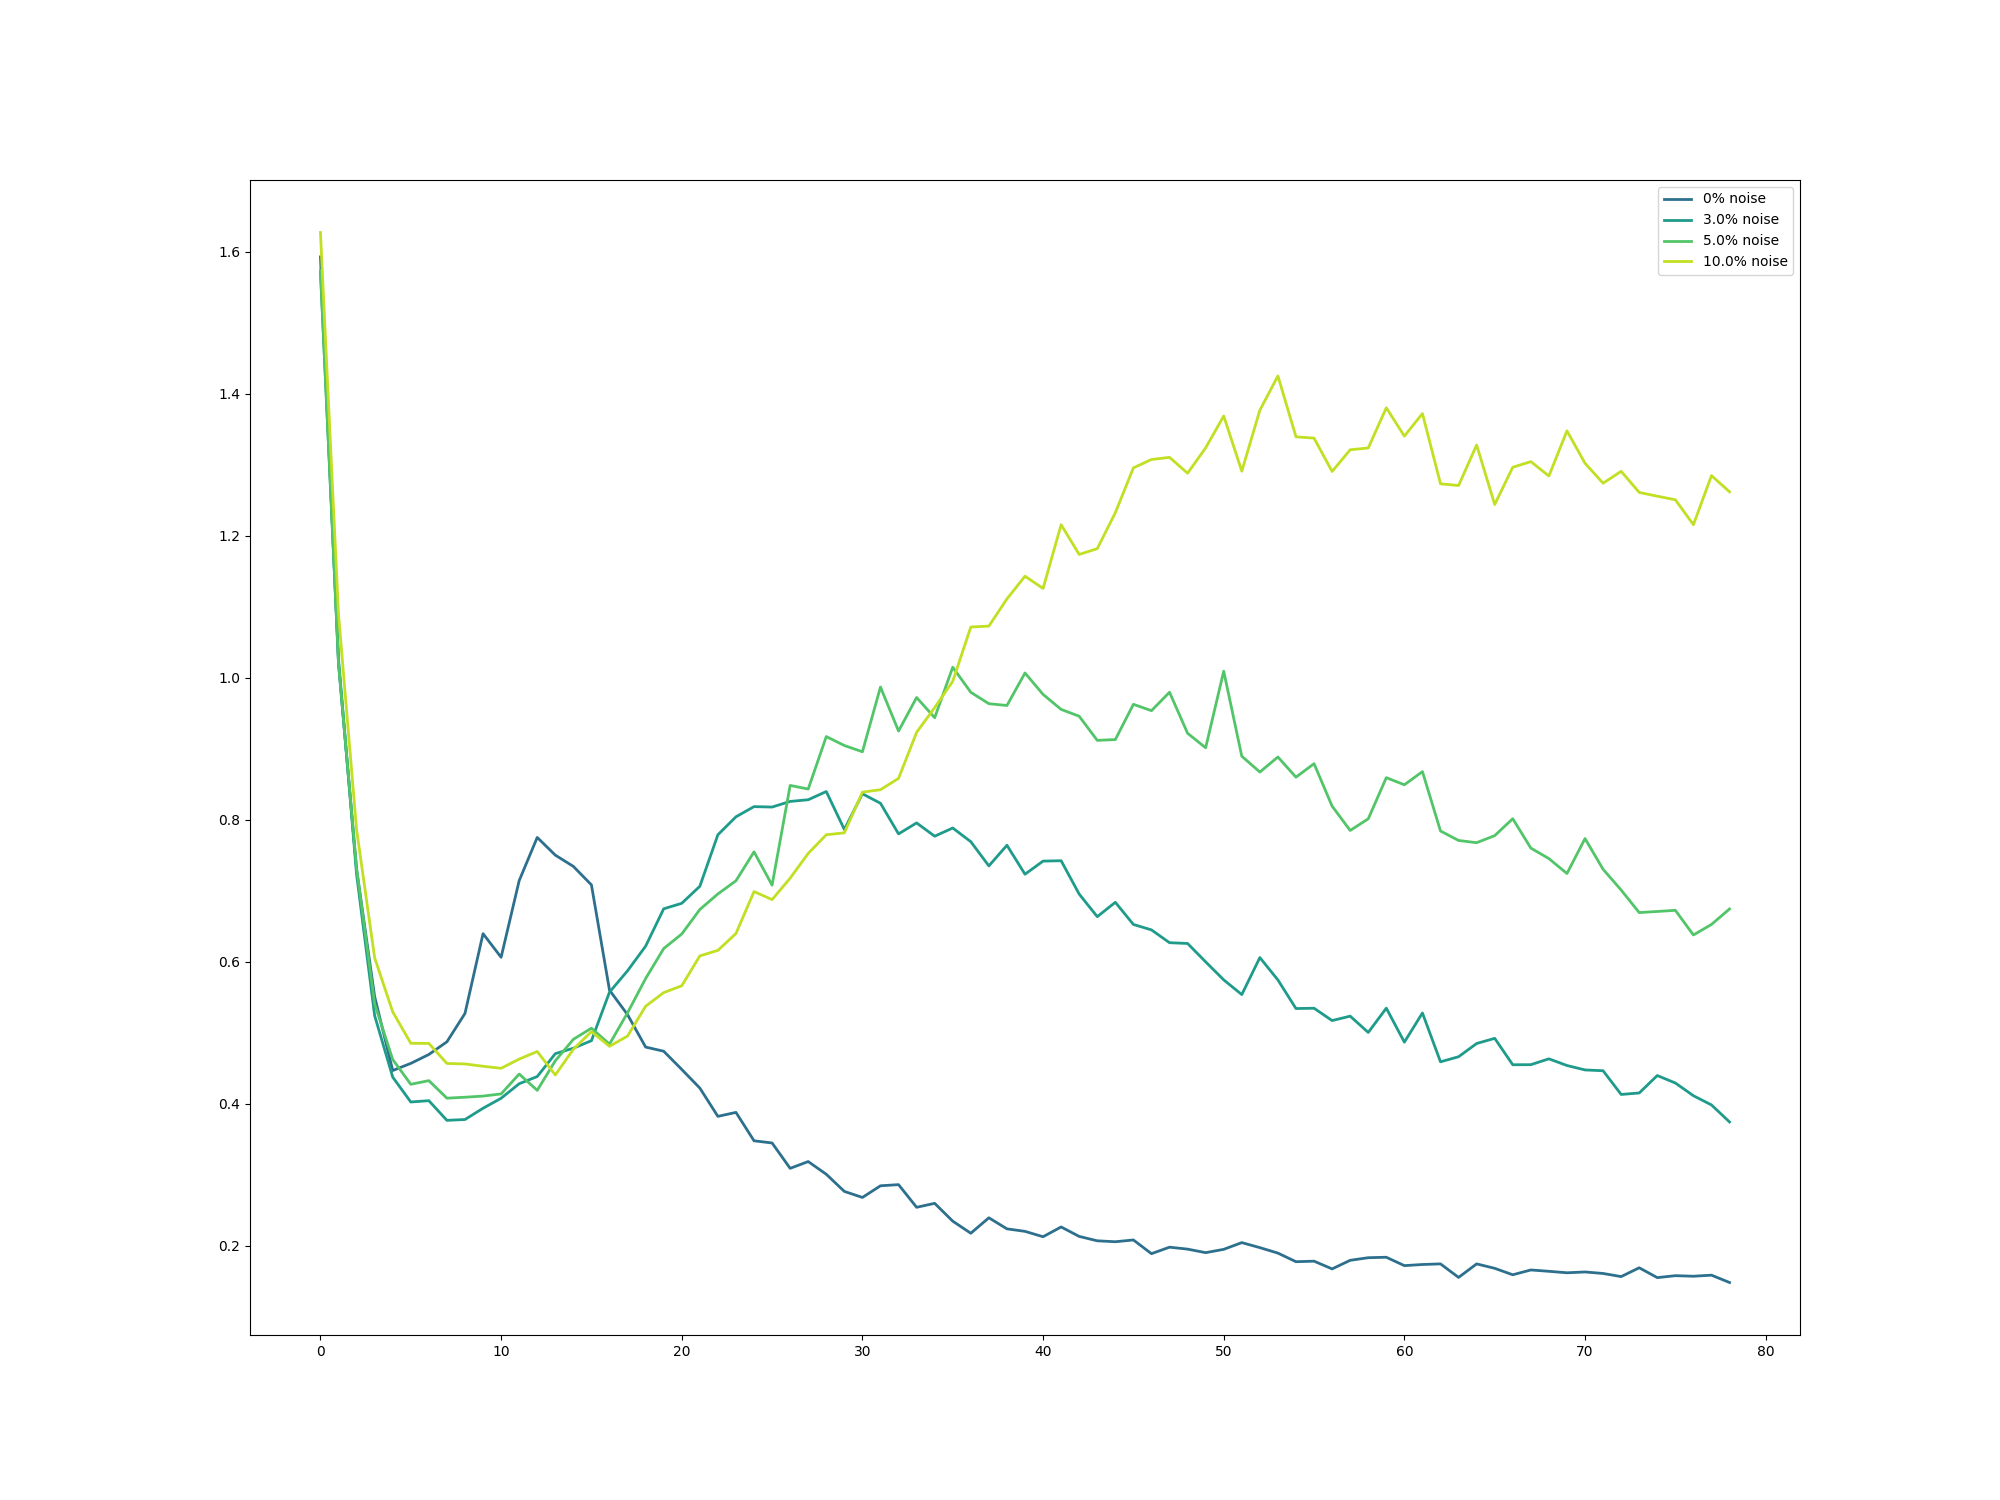
\includegraphics[width= 1\linewidth]{Abschlussarbeit_2021/LaTeX/images/many_curves_less_noise.png}
\caption{Test-loss with different label noise averaged over 4 runs. For the experiment noise was added to the labels. This means, that for a certain probability the label was chosen randomly. The probabilities for each curve is given in the legend.}
\label{fig:Label_noise_on_double_descent}
\end{figure}

%%%%%%%%%%%%%%%%%%%%%%%%%%%%%%%%%%%%%%%%%%%
%%%%%%%%%%%%%%%%%%%%%%%%%%%%%%%%%%%%%%%%%%%
%%%%%%%%%%%%%%%%%%%%%%%%%%%%%%%%%%%%%%%%%%%

\newpage
\section{Double Descent with Optimizer and Data sets}

In the previous experiments, the models were always trained with stochastic gradient descent (SGD). 
Double descent is not only a phenomenon that occurs when training with SGD. The peak can also be seen when training with the ADAM algorithm.
Figure \ref{fig:double_descent_on_optimizers} shows that the peak at the interpolation threshold can also be clearly observed. 

\begin{figure}[!htp]
\centering
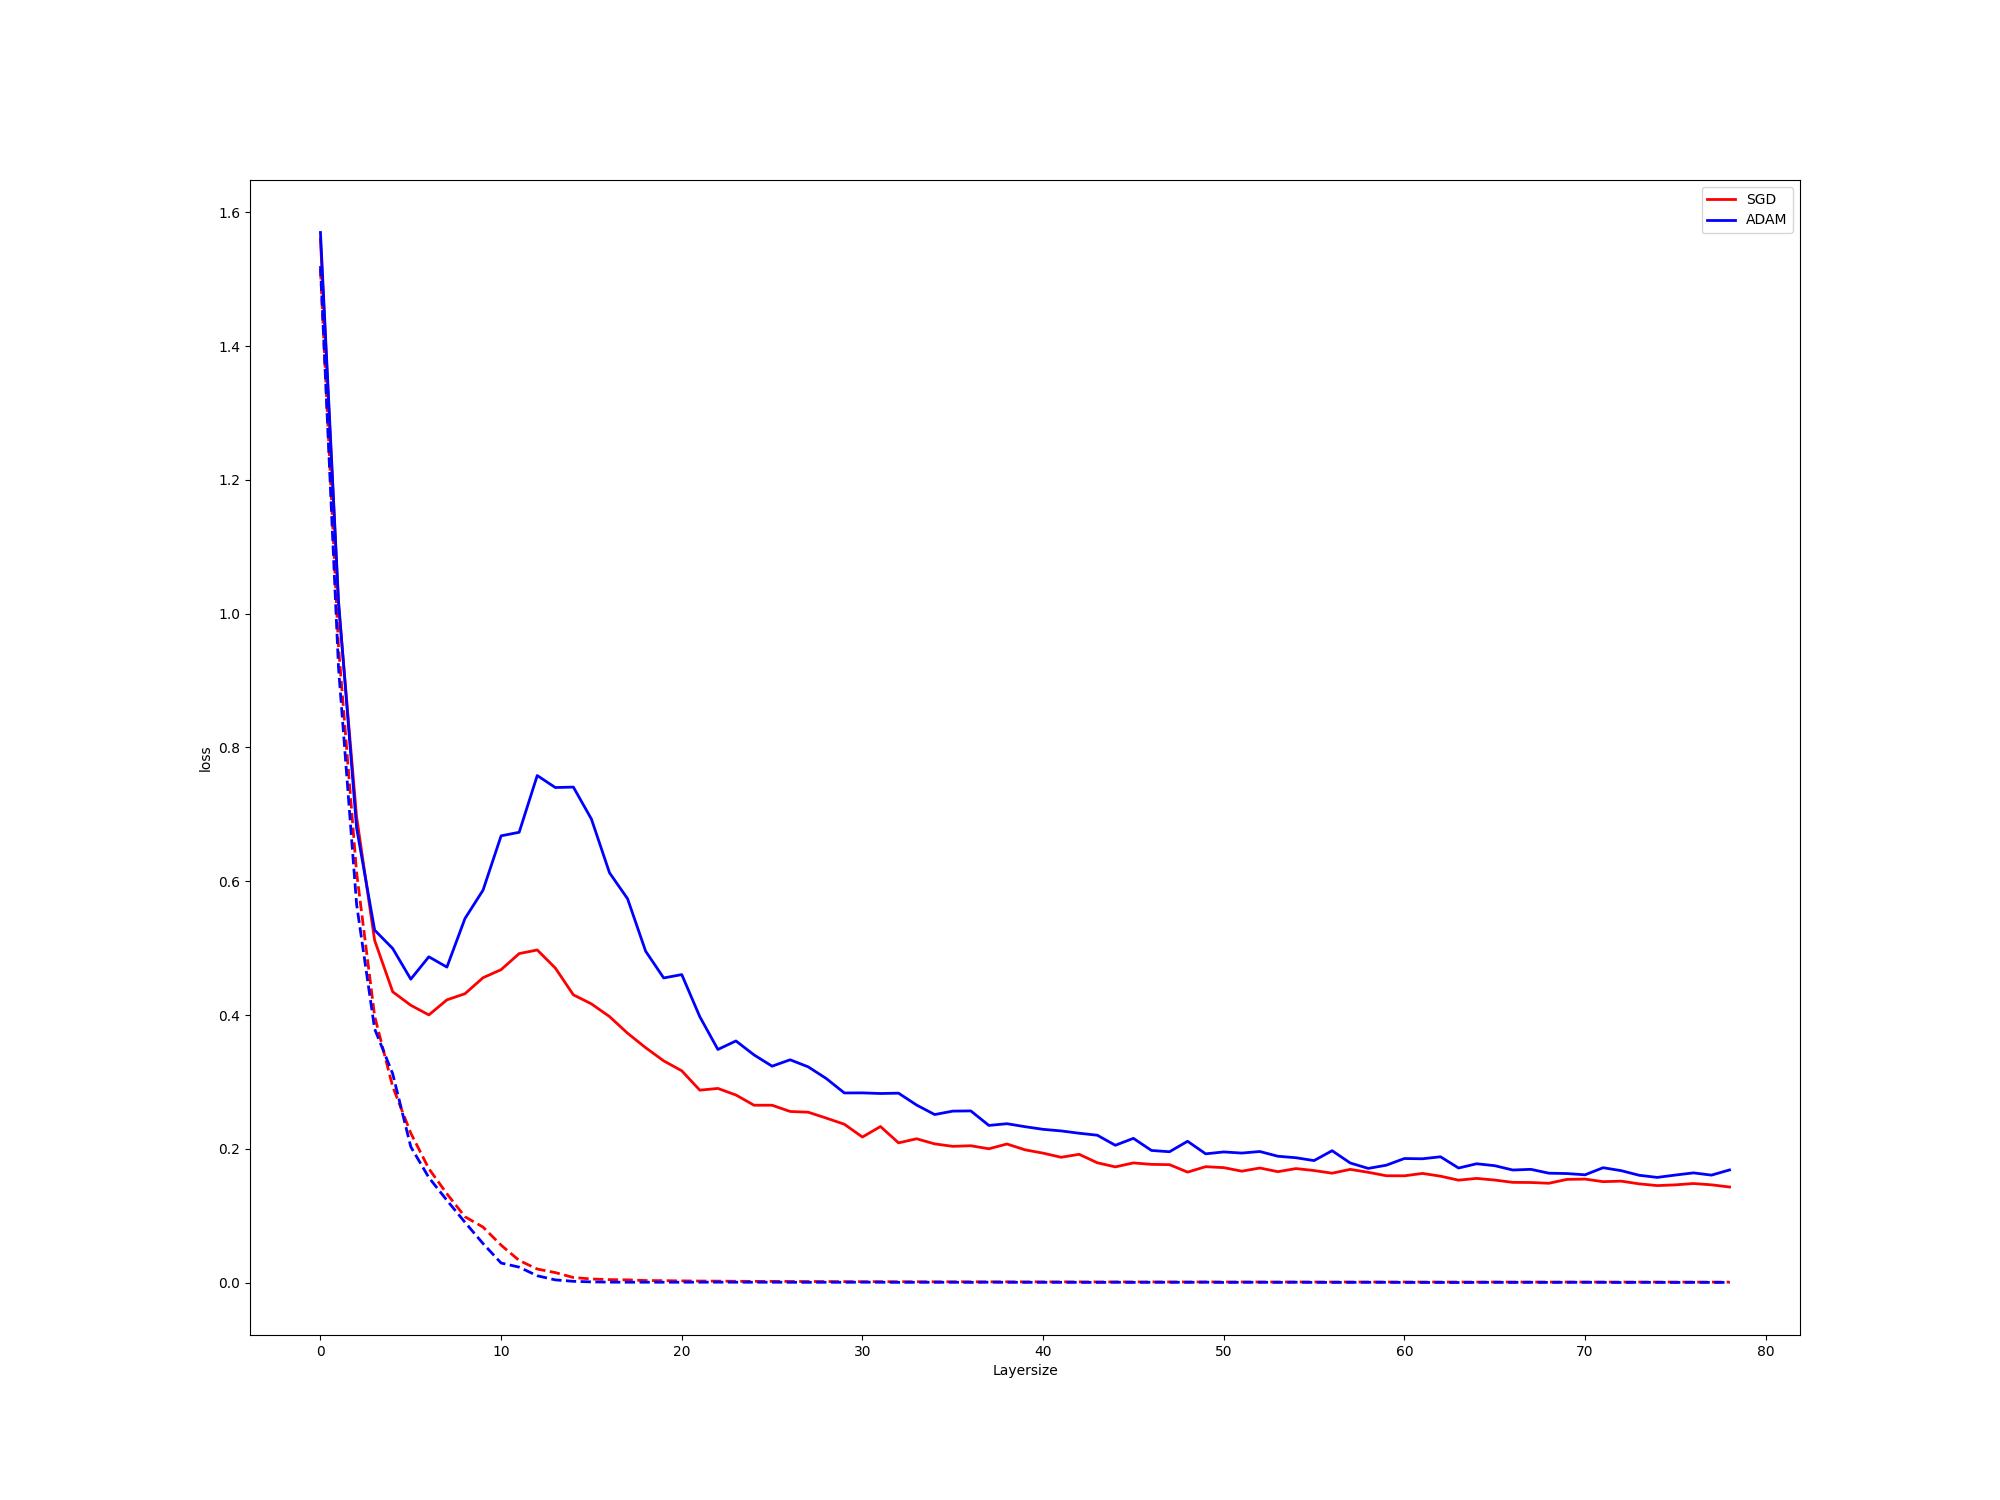
\includegraphics[width= 1\linewidth]{Abschlussarbeit_2021/LaTeX/images/ADAM_vs_SGD.png}
\caption{train and test loss from ADAM and SGD. averaged over 4 runs}
\label{fig:double_descent_on_optimizers}
\end{figure}

One difference between the adam-optimizer and SGD is that the learning rate varies with adam. In SGD this is not the case without instruction. The red curve of the model trained with SGD in \ref{fig:double_descent_on_optimizers} was generated by a learning rate of $\eta = 0.05$. Figure \ref{fig:learning_rates_double_descent} shows that by changing the learning rate $\eta$ the peak of the curve can be changed. Thus, at a higher learning rate, the test loss at the interpolation threshold is significantly higher than at a lower learning rate. If $\eta$ is small enough, it is even possible that no double descent can be seen, unless the model was trained without label noise. The surprisingly high peak, which occurred when using adam, can also be generated with SGD if the learning rate is appropriate. \\
The graph looks similar to the ones in Figure \ref{fig:epochs_double_descent} where the epochs where varied. This might due to the effect, that higher learning rate and processing more epochs have a similar effect on weight change. We will deepen this in Chapter \ref{possible_explanations}. 

\begin{figure}[!htp]
\centering
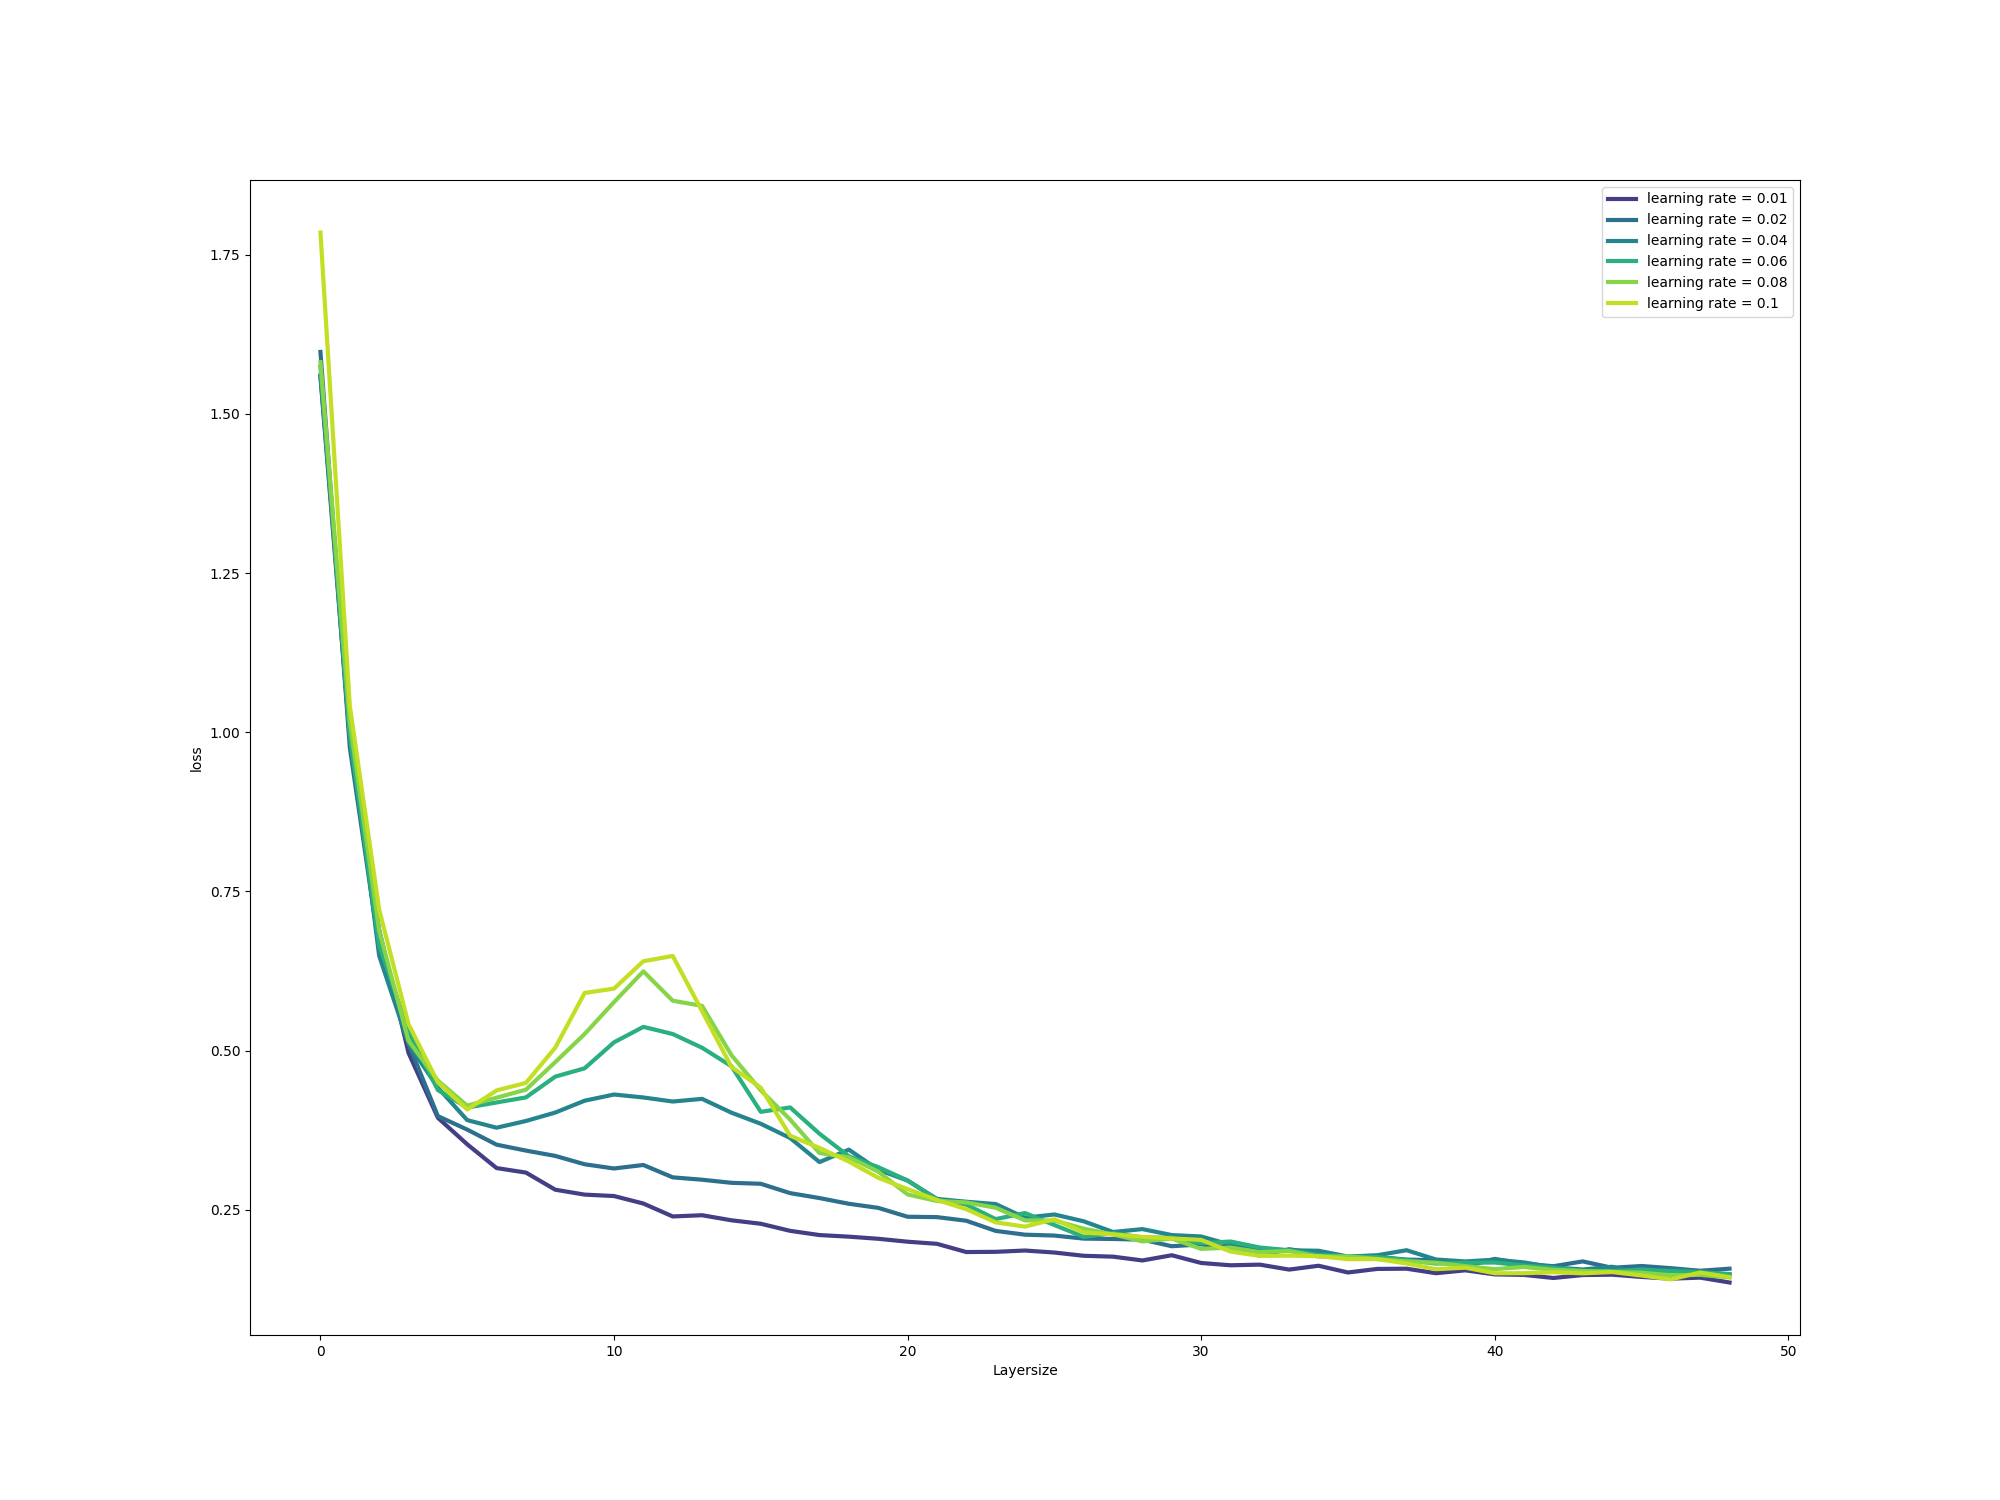
\includegraphics[width= 1\linewidth]{Abschlussarbeit_2021/LaTeX/images/different_learningrates.png}
\caption{test-loss with different learning rates. The curves where averaged over 6 runs. A higher learning rate $\eta$ results in a higher peak at the interpolation threshold}
\label{fig:learning_rates_double_descent}
\end{figure}

\subsubsection{Double descent with different architecture}
To demonstrate that double descent can occur with other loss functions, data sets, and network architectures, a regression problem has been treated in Figure \ref{fig:double_descent_wine} Here the loss function mean squared error (MSE) was used, which is given by,

\begin{equation}
    MSE = \frac{1}{n}\sum_{i=1}^{n}(f(x_i) - y_i)^2
    \label{mse_eq}
\end{equation}

Where $x_i \in X$ is a training point, $y_i$ the corresponding label and $f(x)$ is the function which is represented by the model. This time two fully connected hidden layers were used. The layer size in Figure \ref{fig:double_descent_wine} indicates the size of both hidden layers. The number of weights to be learned increases much faster this time. A set of about 1600 red wines with 11 attributes each was used as data set \cite{wine_data}. The determination of the quality of the wine should be learned by the model. 


\begin{figure}[!htp]
\centering
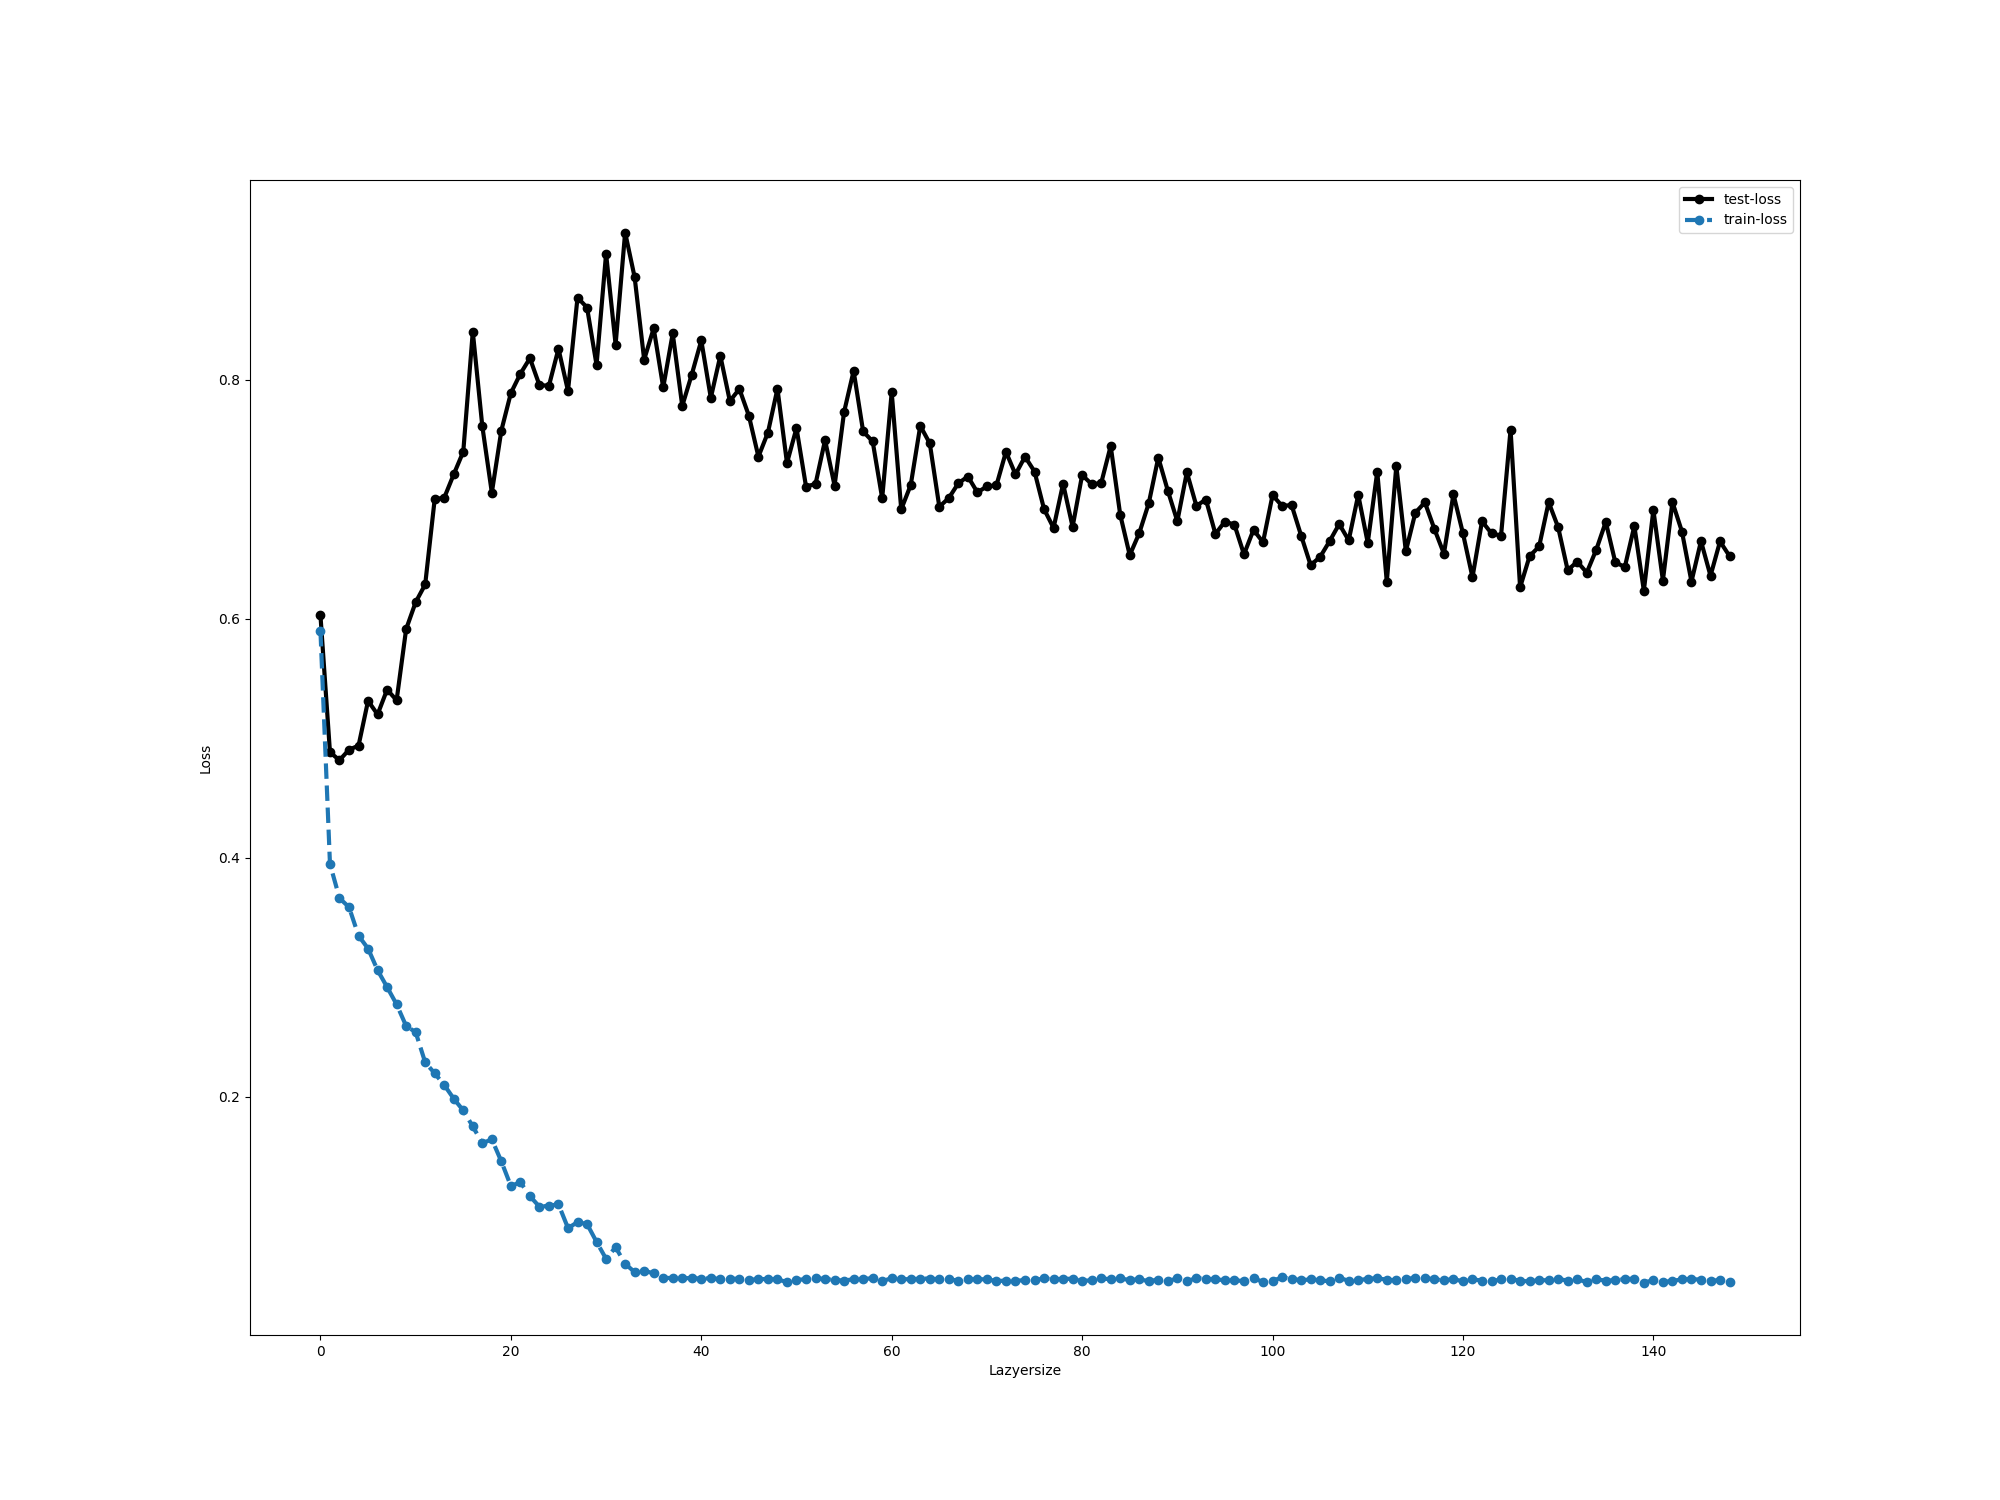
\includegraphics[width= 1\linewidth]{Abschlussarbeit_2021/LaTeX/images/double_descent_regression.png}
\caption{The loss was averaged over 5 runs. The loss at the interpolation threshold $(H \approx 35)$ is even larger than when one neuron is used in both layers. The performance after the interpolation threshold seems to be a lot worse as in the underparametrisized regime. Thus, it can be observed that the performance is not always better far in the overparameterized regime.}
\label{fig:double_descent_wine}
\end{figure}

\section{Observations Summary}

In following lines, we summarize what was observed in the previous experiments.
The following question will be addressed. To what extent is the behavior of the curve predictable if certain parameters are known?\\
The slope around the interpolation threshold, which is typical for the double descent risk curve, can therefore be traced back to different parameters. The peak of this slope is exactly where the training error reaches the value zero (\ref{double_descent_vanilla}).Therefore this peak receives the name "interpolation threshold". The peak takes higher values with stronger overfitting. Overfitting happens with a higher number of epochs, high learning rate or with more noise in the data set.  (\ref{fig:epochs_double_descent}, \ref{fig:Label_noise_on_double_descent}, \ref{fig:learning_rates_double_descent}). The larger $H$ is at the interpolation threshold, the wider is the slope around the interpolation threshold.  This is caused by larger sample size (\ref{fig:sample_size_double_descent}), increased noise (\ref{fig:Label_noise_on_double_descent}) or smaller number of epochs (\ref{fig:epochs_double_descent}). \\
With lower noise, there is a point where over-parameterized networks perform better than smaller under-parameterized ones. This is however not always the case. For example, for the wine quality data set, the test loss in the overparameterized region was significantly worse (\ref{fig:double_descent_wine}) than in the underparameterized region. So using the largest possible network and interpolating all the data is not necessarily the best solution. It is also important to note that the network architecture and the choice of parameters are not optimal for the best possible performance.\\
It was also found that the double descent phenomenon can occur with different network architectures, optimizers, data sets and loss functions. It is therefore worthwhile to investigate the phenomenon further.
Possible reasons why changing the attributes has the described effect will be taken up again in chapter \ref{Discussion}. After the phenomenon is further investigated with various experiments.


